% -----------------------------------------------------------------------------
% Biblioteca de Componentes
% -----------------------------------------------------------------------------

\chapter{Biblioteca de componentes}
\label{chap:bibComponentes}

Conforme mencionado no \autoref{chap:metodologia} deste trabalho, foi proposta a criação de uma pequena biblioteca de componentes como protótipo para um possível \textit{design system} da empresa avaliada no experimento. Essa biblioteca seria construída a partir das definições de design tomadas para um projeto paralelo, intitulado \textit{DitoFeras}. O objetivo de tal projeto é administrar a gestão de colaboradores da empresa, sistema inexistente na organização até então.

Como forma de se iniciar a criação do produto, foi executada uma técnica de \textit{brainstorming}, proposta pela metodologia de \textit{design sprint}, conhecida como \textit{Crazy Eights}. Para a execução da técnica, foram envolvidos cinco profissionais da empresa, sendo dois destes designers e os demais desenvolvedores. Tomando como base a ideia de criação de um sistema de gestão de funcionários, cada indivíduo recebeu uma folha de papel dividia em oito seções. O desafio seria preencher, em cinco minutos, cada uma das seções da folha com esboços de interfaces que poderiam compor o sistema aumejado. Ao final do tempo estabelecido, cada participate deveria apresentar e defender suas ideias. A \autoref{fig:crazy8} apresenta um dos exemplos de esboços construídos durante o procedimento.

\begin{figure}
	\frame{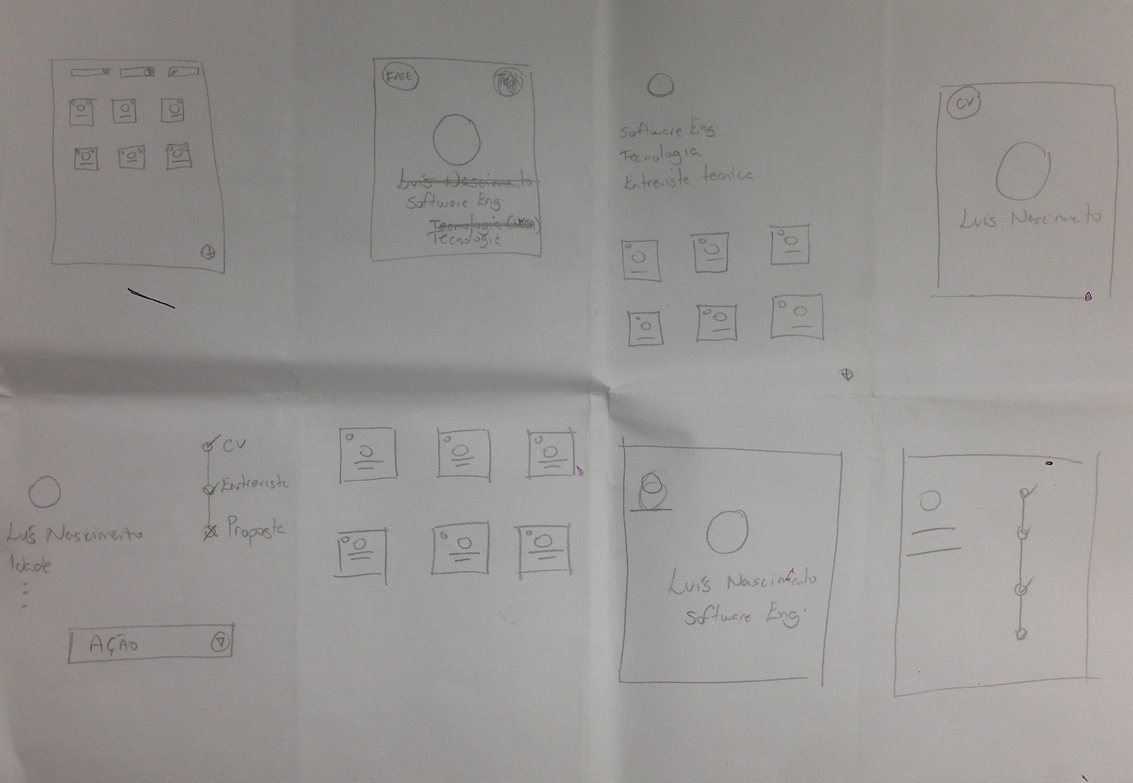
\includegraphics[width=\linewidth]{./04-figuras/06_biblioteca_componentes/crazy8.jpg}}
  \caption{Exemplo de artefato do \textit{Crazy Eights}}
  \fonte{Próprio autor}
  \label{fig:crazy8}
\end{figure}

A atividade de \textit{brainstorming} foi de fato um sucesso, gerando como saída vários artefatos e ideias que serviram de gatilho para o novo produto. Durante o processo, foram definidos os primeiros entregáveis: uma tela de \textit{login} e uma tela de listagem de funcionários.

Partiu-se, enfim, para a criação da biblioteca de componentes que seria utilizada como base para o desenvolvimento do novo sistema. Seguindo a ideia da Ryte \cite{ryteDesignSystem}, optou-se por dividir a biblioteca de componentes em dois grandes artefatos: um guia de design e um repositório com as implementações dos componentes.

A \autoref{fig:figma} ilustra a estrutura do guia de design produzido, já a \autoref{fig:sourceTree} apresenta a estrutura de arquivos do repositório que concentra as implementações dos componentes. Foi utilizado o Figma como ferramenta de criação do guia de design e o Angularjs como \textit{framework} base para implementação dos componentes. Percebe-se certa semelhança na forma como são organizadas as estruturas internas de cada artefato. Tal semelhança é reflexo do processo de co-criação do produto, onde os envolvidos no projeto tiveram participação ativa durante todo o processo, utilizando as mesmas terminologias para se referir aos componentes.

\begin{figure}
	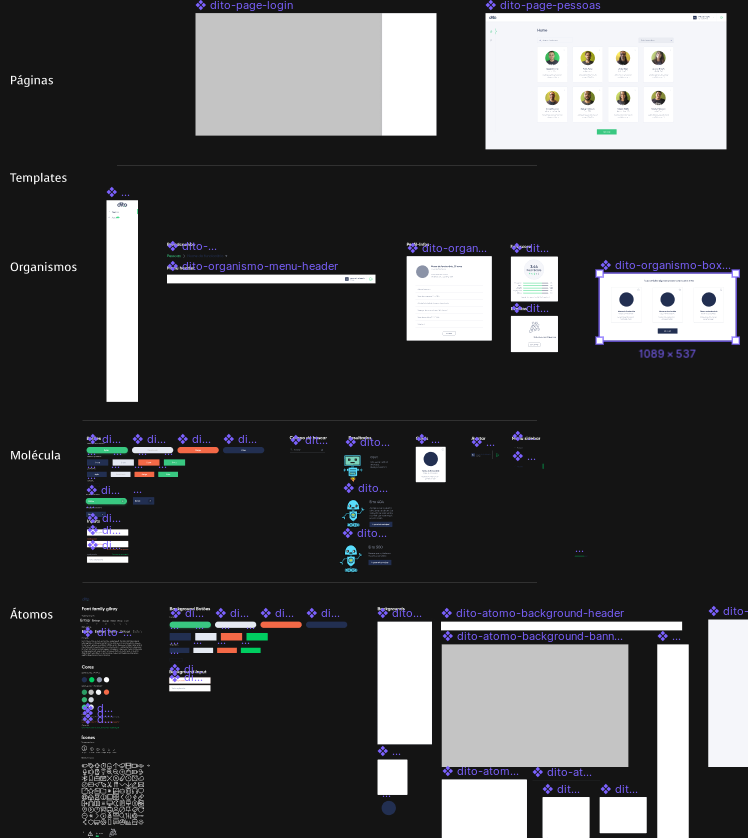
\includegraphics[width=\linewidth]{./04-figuras/06_biblioteca_componentes/styleguide-figma.png}
  \caption{Estrutura da biblioteca de componentes no Figma}
  \fonte{Próprio autor}
  \label{fig:figma}
\end{figure}

\begin{figure}
  \begin{center}
	  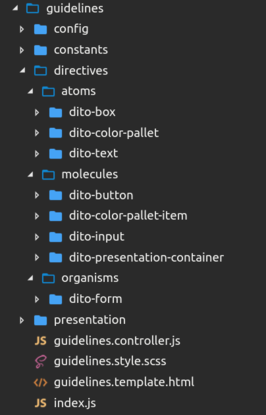
\includegraphics[]{./04-figuras/06_biblioteca_componentes/source-tree.png}
	\end{center}
  \caption{Árvore de diretórios da biblioteca de componentes}
  \fonte{Próprio autor}
  \label{fig:sourceTree}
\end{figure}

Seguindo a metodologia do \textit{Atomic Design} \cite{frostAtomicDesign}, os componentes do sistema foram construídos em uma estrutura \textit{bottom-up}, ou seja, do componente mais simples para o mais complexo. A seguir são apresentadas a anatomia de alguns dos componentes presentes no sistema.

\section{Átomos}

Os átomos são representações dos blocos básicos para a contrução de componentes mais complexos do sistema. O \autoref{table:atomsDitoFeras} apresenta o que foi entendido como átomo do sistema, além de descrever seu propósito.

\begin{quadro}
\centering
\begin{tabular}{|m{4cm}|m{10cm}|} \hline
	
	\multicolumn{1}{|c|}{\bfseries Nome} & \multicolumn{1}{c|}{\bfseries Descrição} \\\hline
	
	 \textit{dito-box} &  Representa um container de conteúdos. \\\hline
	 
	 \textit{dito-color-pallet} & Paleta de cores da aplicação. Padroniza o espectro de cores a ser utilizado ao longo do sistema. \\\hline
	 
	 \textit{dito-text} & Consolida os tipos de textos presentes no sistema. Deve abrangir semânticamente títulos, parágrafos, \textit{placeholders} e etc. Padroniza tamanhos de fonte, família da fonte, intensidade do texto e etc. \\\hline
    
\end{tabular}
\caption{Átomos do sistema \textit{DitoFeras}}
\fonte{Próprio autor}
\label{table:atomsDitoFeras}
\end{quadro}

Dos átomos listados, a paleta de cores é aquele que apresenta maior destaque, sendo de fundamental importância para garantir consistência na experiência do usuário ao utilizar o sistema. A \autoref{fig:colorPallet} apresenta a implementação desse componente.

\begin{figure}
  \begin{center}
	  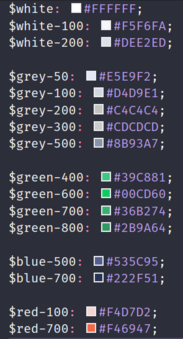
\includegraphics[]{./04-figuras/06_biblioteca_componentes/color-pallet.png}
	\end{center}
  \caption{Paleta de cores do sistema \textit{DitoFeras}}
  \fonte{Próprio autor}
  \label{fig:colorPallet}
\end{figure}

Percebe-se que a implementação do átomo da paleta de cores se restringe a um arquivo \textit{SASS} com definições de cores em variáveis. Não deve haver, ao longo das implementações dos outros componentes, nenhuma atribuição de cor que não utilize as variáveis definidas por este átomo.

\section{Moléculas}

As móleculas são conjuntos de átomos que, combinados, geram um valor mínimo para o usuário final. O \autoref{table:moleculesDitoFeras} apresenta o que foi entendido como mólecula do sistema, além de descrever seu propósito.

\begin{quadro}
\centering
\begin{tabular}{|m{4cm}|m{10cm}|} \hline
	
	\multicolumn{1}{|c|}{\bfseries Nome} & \multicolumn{1}{c|}{\bfseries Descrição} \\\hline
	
	 \textit{dito-button} & Abstração dos possíveis botões do sistema. \\\hline
	 
	 \textit{dito-color-pallet-item} & Representa a forma apresentável de uma cor da paleta de cores. Inclui, além da cor em si, seu nome e sua representação em hexadecimal. \\\hline
	 
	 \textit{dito-input} & Abstração dos possíveis campos de entrada de texto do sistema. \\\hline
	 
	 \textit{dito-presentation-container} & Representa um container de componentes. Utilizado nas páginas de apresentação da biblioteca de componentes. \\\hline
    
\end{tabular}
\caption{Moléculas do sistema \textit{DitoFeras}}
\fonte{Próprio autor}
\label{table:moleculesDitoFeras}
\end{quadro}

Das moléculas listadas, o componente de botões é aquele que vale ser ressaltado. Diferentemente da simplicidade dos átomos, móleculas são componentes mais complexos e normalmente abstraem algum tipo de comportamento internamente. O \autoref{table:ditoButton} apresenta a anatomia do \textit{dito-button}, descrevendo sua interface de uso.

\begin{quadro}
\centering
\begin{tabular}{|m{4cm}|m{3cm}|m{7cm}|} \hline
	
	\multicolumn{1}{|c|}{\bfseries Atributo} & \multicolumn{1}{c|}{\bfseries Tipo} & \multicolumn{1}{c|}{\bfseries Descrição} \\\hline
	
	 \textit{type} & \textit{string} & Define o tipo do botão. São reconhecidos dois tipos: padrão e envio (\textit{submit}). Caso não informado, assume-se o valor padrão. \\\hline
	 \textit{onClick} & \textit{function} & Função que será executada após algum evento de clique por parte do usuário. \\\hline
	 \textit{isDisabled} & \textit{boolean} & Informa se o botão está em um estado desabilitado, ou não. Quando desabilitado, ações de clique, por parte do usuário, são ignoradas. \\\hline
    
\end{tabular}
\caption{Interface de uso do componentes \textit{dito-button}}
\fonte{Próprio autor}
\label{table:ditoButton}
\end{quadro}

Pode-se perceber que o componentes \textit{dito-button} possui um mecanismo de estado associado. Dessa forma, o comportamento do componente depende diretamente do estado atual do mesmo. A \autoref{fig:buttons} ilustra o componente nos seus seis diferentes tipos de estado.

\begin{figure}
  \begin{center}
	  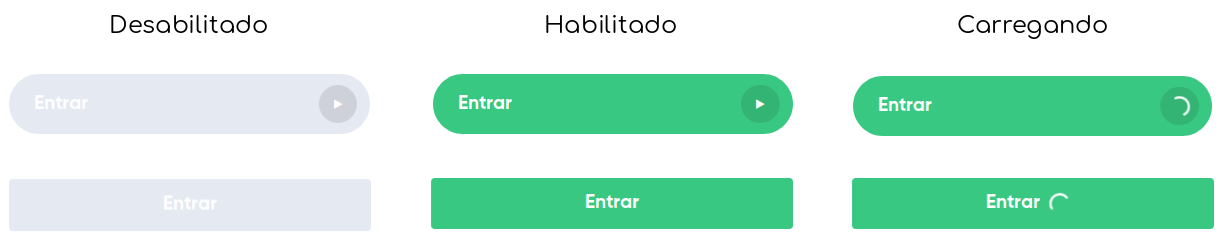
\includegraphics[width=\linewidth]{./04-figuras/06_biblioteca_componentes/buttons.png}
	\end{center}
  \caption{Estados de um botão do sistema \textit{DitoFeras}}
  \fonte{Próprio autor}
  \label{fig:buttons}
\end{figure}

\section{Organismos}

Organismos são grupos de moléculas que, juntas, formam uma seção relativamente complexa e distinta da interface de usuário. Até o momento em que o presente trabalho foi escrito, o único organismo implementado no sistema foi o \textit{dito-form}, que encapsula lógicas de validação de formulários de envio de dados para o servidor. A \autoref{fig:forms} ilustra um formulário de \textit{login} em três diferentes estados.

\begin{figure}
  \begin{center}
	  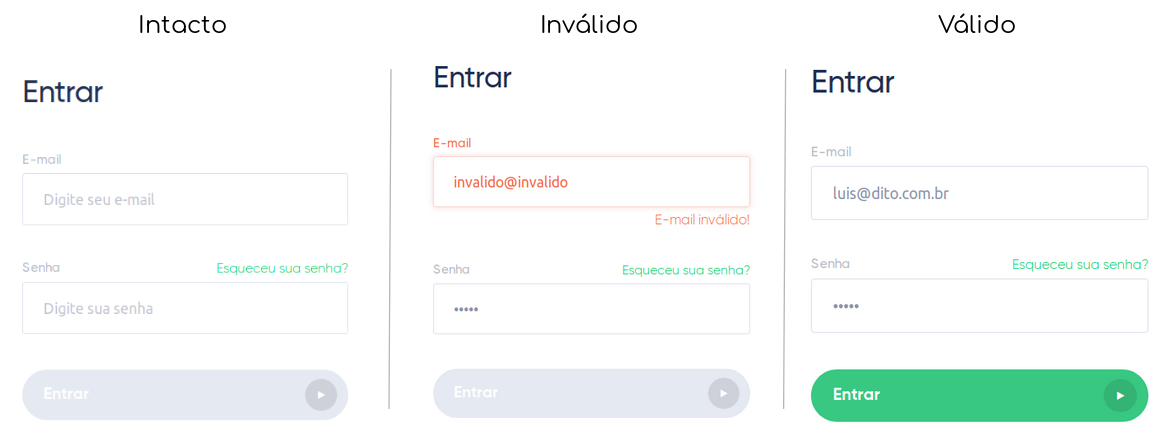
\includegraphics[width=\linewidth]{./04-figuras/06_biblioteca_componentes/forms.png}
	\end{center}
  \caption{Estados de um formulário de \textit{login} do sistema \textit{DitoFeras}}
  \fonte{Próprio autor}
  \label{fig:forms}
\end{figure}

Por estratégia do autor, não foram implementadas as abstrações de templates proposta pela metodologia do \textit{atomic design}, uma vez que a reusabilidade de páginas seria mínima em um estágio inicial de projeto.

No capítulo seguinte serão apresentadas as páginas implementadas do sistema que utilizaram a biblioteca de componentes ilustrada neste capítulo como blocos básicos de sua construção.